
% !TeX document-id = {b30d14d7-2607-4df4-a1ff-fee288478bc5}
% !TeX spellcheck = it_IT
% !TeX root = UsoMail.tex

\documentclass[structure=book,  
pagelayout=standard,defaultfont=cochineal,partialtoc]{suftesi}
\usepackage{fontspec}
\usepackage{polyglossia}
\setmainlanguage{italian}
\setotherlanguage{english}
\title{Le utenze di Workspace}
\author{Claudio Duchi}
\date{\today}
\usepackage{booktabs}
\usepackage{imakeidx}
\makeindex[intoc]
\newcommand{\printmail}[1]{\textbf{#1}}
\usepackage[style=italian]{csquotes}
\usepackage[%
style=philosophy-modern,
backend=biber]{biblatex}
\addbibresource{UsoMail.bib}
\partialtocsize{\footnotesize}
\partialtocsecfont{\bfseries\itshape}
\partialtocsubsecfont{\itshape}
\partialtocseclabel{\bfseries}
\partialtocbeforecode{\hrule\smallskip\textbf{Contents}\smallskip}
\partialtocaftercode{\smallskip\hrule}
\usepackage{hyperref}
% !TeX spellcheck = it_IT
% !TeX root = UsoMail.tex
\includeonly{mailistituzionale,Buonepratiche,GoogleWorkspace,unitaorganizzative}
\begin{document}
\maketitle
\colophon{Claudio Duchi}{}
\tableofcontents
\listoftables

% !TeX spellcheck = it_IT
% !TeX root = UsoMail.tex
\begin{changelog}[author=JOHN DOE, sectioncmd=\chapter*]
	\begin{version}[v=1.9.9,
		date=2023-08-25]
		\added
		\item Revisionato fino a gruppi compreso
		\fixed
		\item Bug fixes
	\end{version}
	\begin{version}[v=1.0.6,
		date=2023-08-14]
		\added
		\item Aggiunta composizione gruppi dipartimentali
		\fixed
		\item Bug fixes
	\end{version}
	\begin{version}[v=1.0.5,
		date=2023-08-11]
		\added
		\item Descrizione utente e suoi attributi
		\fixed
		\item Bug fixes
	\end{version}
	\begin{version}[v=1.0.4,
		date=2023-07-25]
		\added
		\item Spostamenti classi
		\fixed
		\item Bug fixes
	\end{version}
	\begin{version}[v=1.0.3,
		date=2023-07-25]
		\added
		\item Regole mail
		\fixed
		\item Bug fixes
	\end{version}
		\begin{version}[v=1.0.2,
		date=2023-07-21]
		\added
		\item Meet
		\item Permettere a  UA studenti di creare Meet.
		\item Permettere a UA studenti di ammettere nelle riunioni utenti esterni alla scuola.
		\fixed
		\item Bug fixes
	\end{version}
	\begin{version}[v=1.0.1,
		date=2023-07-17]
		\added
		\item Fine Anno prima versione
		\item Inserire nuovi utenti con modifica password
		\fixed
		\item Bug fixes
	\end{version}
	\begin{version}[v=1.0.0,
		date=2023-07-15]
		\added
		\item Massive upgrade
		\item Sospendere e spostare
		\fixed
		\item Bug fixes
	\end{version}
		\shortversion{v=0.0.1,
		date=2023-12-13,
		changes=Versione iniziale}
	\end{changelog}
	\listoftodos
% !TeX spellcheck = it_IT
% !TeX root = UsoMail.tex
\chapter{La mail istituzionale}
%\printpartialtoc
\section{Definizioni}
La scuola fornisce ad ogni utente una mail istituzionale\index{Mail!istituzionale} (MI) che permette 
la comunicazione fra gli utenti interni e con entità esterne alla scuola. La MI sostituisce la mail personale dell'utente nei suoi rapporti
da o verso la scuola, permettendo di separare la vita  personale da quella lavorativa.

Ogni mail viene rilasciata utilizzando il seguente schema\index{Mail!istituzionale!schema}:
\begin{itemize}
	\item \printmail{nome.cognome.doc@iisperugia.net} se l'utente è un docente
	\item \printmail{nome.cognome.stu@iisperugia.net} se l'utente è uno studente
	\item \printmail{nome.cognome.tir@iisperugia.net} se l'utente è un 
	tirocinante
	\item \printmail{nome.cognome.ata@iisperugia.net} se l'utente è un 
	assistente 
	amministrativo.
	\item \printmail{nome.cognome.visitatore@iisperugia.net} se l'utente è un 
	utente provvisorio.
\end{itemize}

A una mail corrisponde una password di almeno otto caratteri entrambi permettono
l'accesso ai servizi di  \textenglish{Google Workspace} altrimenti noto come \textenglish{G Suite}.

Il sistema è gestito da amministratori che possono: creare, sospendere, cancellare un'utenza. Possono inoltre, limitare l'uso del sistema a utenti o gruppi di utenze, non possono leggere il contenuto della MI ma controllare se una mail è stata spedita e a chi. Gli amministratori inoltre possono verificare se un utente è entrato nel sistema e leggere i file log del sistema.

\section{Regole di creazione} 
La mail viene rilasciata dagli amministratori del sistema utilizzando le seguenti 
regole:

Se l'utente ha un solo cognome e un solo nome viene creato
\begin{center}
	\printmail{nome.cognome.doc@iisperugia.net}
\end{center}
esempio: Mario Rossi, docente avremo:
\begin{center}
	\printmail{mario.rossi.doc@iisperugia.net}
\end{center}
Se una persona ha più di un nome o di un cognome si usa il primo nome e il  
primo cognome: Carlo Mario Bianchi Rossi studente diventa
\begin{center}
	\printmail{carlo.bianchi.stu@iisperugia.net}
\end{center}
In caso di omonimia viene aggiunto un numero dopo il cognome.
\section{Mail istituzionale e Privacy}
Partiamo da qualche osservazione: la mail è inviolabile, la 
MI è uno strumento di lavoro. L'utente deve impegnarsi a controllarla perché questa permette la comunicazione fra lui e la scuola. 

La MI è 
un dato sensibile, per proteggere la privacy del titolare,  sono quindi 
disponibili delle mail alias~\footcite{Garante2007}\index{Mail!istituzionale!alias} che nascondono l'identità di utenti 
che  hanno rapporti 
con l'esterno dell'organizzazione~\footnote{segreteria@iisperugia.net, pcto@iisperugia.net}. 



Per garantire la privacy dell'utente, la scuola fornendo questo servizio, non può, salvo casi eccezionali, utilizzare 
la mail personale dell'utente.

L'utente non può a sua volta utilizzare la MI per  usi  
personali dato il profilo istituzionale di questa. 

 All'inizio del rapporto con la scuola, l'utente dovrebbe essere informato di questo 
in modo da non portare a fraintendimenti in futuro.

Il Garante della privacy~\footcite{Garante2007}\index{Garante della privacy} chiede che 
venga definito un disciplinare, noto agli utenti, che spieghi le procedure con cui vengono la MI. 
L'utente deve conoscere il percorso di vita della sua utenza, creazione, uso, 
recupero eventuale di dati, 
cancellazione~\footcite{Garante2007}~\footcite{Garante2019}. 

L'utente deve 
essere consapevole che 
può recuperare i propri dati trasferendo  la sua utenza. 

La MI permette l'utilizzo all'utente delle varie applicazioni che formano \textenglish{Google Workspace}
\section{Alias}
Un'email\index{Mail!alias} alias è una mail di inoltro che viene aggiunta dall'amministratore ad un utente\footcite{Google2023d} tramite console\index{Console!amministrazione!alias}. Tale mail non può essere condivisa ne è un account.
L'amministratore può creare fino a trenta alias diversi per utente.
\begin{center}
	
\begin{tabular}{lll}
	\toprule 
	Titolo&Nome&Mail Alias\\
	\midrule
	Animatore digitale&
	Danilo Ardillo&
	animatore@iisperugia.net\\
	Bullismo Madonna Alta&
	Matteo Castellini&
	bullismomalta@iisperugia.net\\
	Bullismo Olmo&
	Amelia Sabatino&
	bullismoolmo@iisperugia.net\\
	Corso Serale&
	Daniela Strona&
	serale@iispeugia.net\\
	Disciplinare&
	Alessia Nunzi&
	disciplinare@iisperugia.net\\
	Educazione Civica&
	Angela Longo&
	civica@iisperugia.net\\
	Erasmus+&
	Lucia Cozzolino&
	erasmus@iisperugia.net\\
	Invalsi&
	Marisa Pettirossi&
	invalsi@iisperugia.net\\
	PCTO manutenzione&
	Marco Biccheri&
	pctomanutenzione@iisperugia.net\\
	PCTO moda&
	Paola Viscuso&
	pctomoda@iisperugia.net\\
	PCTO Olmo&
	Stefano Rossi Ciucci&
	pctoolmo@iisperugia.net\\
	PCTO Pascal&
	Annalisa Cicioni&
	pctopascal@iisperugia.net\\
	Pon e Formazione&
	Danilo Ardillo&
	pon@iisperugia.net\\
	Referente corso elettronica&
	Pasquale Costanzo&
	corsoe@iisperugia.net\\
	Referente corso gestione acque&
	Moretti Orietta&
	corsog@iisperugia.net\\
	Referente corso meccanica&
	Francesco Dottori&
	corsot@iisperugia.net\\
	Referente corso moda&
	Paola Viscuso&
	corsoa@iisperugia.net\\
	Referente corso servizi commerciali&
	Antonella Pesce&
	corsob@iisperugia.net\\
	Referente Dsa/altroBes&
	Simonetta Tini&
	dsabes@iispeugia.net\\
	Referente Inclusione&
	Annalisa Federici&
	rinclusione@iisperugia.net\\
	Sostegno Madonna Alta&
	Annalisa Federici&
	sostegnomalta@iisperugia.net\\
	Sostegno Olmo&
	Stefania Pedini&
	sostegnoolomo@iisperugia.net\\
	Sostegno Piscille&
	Elisa Castellani&
	sostegnopiscille@iisperugia.net\\
	Supervisore Google Workspace &
	Danilo Ardillo&
	supervisore@iisperugia.net\\
	Supervisore Google Workspace Madonna Alta&
	Annalisa Cicioni&
	supervisoremalta@iisperugia.net\\
	Supervisore Google Workspace Olmo&
	Bryan Balingit&
	supervisoreolmo@iisperugia.net\\
	Supervisore Google Workspace Piscille&
	Claudio Duchi&
	supervisorepiscille@iisperugia.net\\
	Viaggi di istruzione e visite didattiche&
	Daniela Strona&
	viaggi@iispeugia.net\\
	\bottomrule
\end{tabular}
\captionof{table}{Alias attivi}
\end{center}
\begin{figure}
	\centering
	\begin{forest}
	[Utente[Mail Istituzionale][Unità organizzativa][Gruppo][Opzionale[Drive][Alias]]]
\end{forest}
	\caption{Descrizione utente e suo attributi}
\end{figure}
% !TeX spellcheck = it_IT
% !TeX root = UsoMail.tex
\chapter{Google Workspace}
%\printpartialtoc
\section{I servizi di Google}
La MI permette,tramite la scuola, l'accesso ai servizi, forniti da \textenglish{Google}, di \textenglish{Google Workspace}. Tali servizi sono regolati da un contratto sottoscritto dalla scuola~\footcite{Google2020}. La versione in uso dalla scuola è:  \textenglish{Google Workspace for Education Fundamentals}.

\textenglish{Google} suddivide i servizi che fornisce in due gruppi "Servizi principali" e in "Servizi aggiuntivi"\footcite{Google2021a}

I "Servizi principali" sono  descritti da \textenglish{Google} in riepilogo dei servizi~\footcite{Google2022d} e sono in gran parte riportando la descrizione:

\begin{quotation}\textenglish{"Gmail"}\index{Gmail} è un servizio email basato sul Web che consente a un'organizzazione di gestire il proprio sistema di posta elettronica utilizzando i sistemi di \textenglish{Google}. Permette all'Utente finale di accedere alla propria casella di posta da un browser web supportato, leggere la posta, scrivere, rispondere a messaggi e inoltrarli, cercare nella posta e organizzarla tramite etichette. Offre inoltre filtri antispam e antivirus e consente agli Amministratori di creare regole per la gestione dei messaggi con contenuti specifici e file allegati o di indirizzare i messaggi ad altri server di posta. È possibile configurare regole per gruppo o per Cliente (tutti i domini).
	\end{quotation}
\begin{quotation}
	\textenglish{"Google Calendar"}\index{Google!Calendar} è un servizio basato sul Web per la gestione di calendari personali, dell'azienda/organizzazione e dei team. Fornisce agli Utenti finali un'interfaccia in cui visualizzare i calendari, pianificare riunioni con gli altri Utenti finali, vedere le informazioni sulla disponibilità degli altri Utenti finali e prenotare stanze e risorse.
\end{quotation}
\begin{quotation}
	"Documenti Google", "Fogli Google", "Presentazioni Google" e "Moduli \textenglish{Google}"\index{Google!Documenti }\index{Google!Fogli}\index{Google!Presentazioni}\index{Google!Moduli} sono servizi basati sul Web che permettono agli Utenti finali di creare, modificare, condividere, disegnare, esportare, incorporare e lavorare in modo collaborativo su contenuti di documenti, fogli di lavoro, presentazioni e moduli.
\end{quotation}
\begin{quotation}
	\textenglish{"Google Drive"}\index{Google!Drive} fornisce strumenti basati sul Web che consentono agli Utenti finali di archiviare, trasferire e condividere file, nonché di guardare video.
\end{quotation}
\begin{quotation}
	 \textenglish{"Google Groups for Business"}\index{Google!Groups for Business} è un servizio basato sul Web che consente agli Utenti finali e ai proprietari di siti web di creare e gestire gruppi di collaborazione. Gli Utenti finali possono intrattenere discussioni via email e condividere documenti, calendari, siti e cartelle con i membri di un gruppo. Inoltre, possono visualizzare gli archivi delle discussioni del gruppo ed eseguire ricerche in questi ultimi.
\end{quotation}
\begin{quotation}
\textenglish{"Google Chat"}\index{Google!Chat} e   \textenglish{"Google Meet"}\index{Google!Meet} sono servizi basati sul Web che consentono agli Utenti finali di comunicare tra loro in tempo reale.
  
	\textenglish{"Google Chat"}\index{Google!Chat} offre una piattaforma avanzata per la messaggistica via chat e la collaborazione in gruppo che supporta le integrazioni di contenuti con servizi di terze parti selezionati. 	
	
	\textenglish{"Google Meet"}\index{Google!Meet} permette di organizzare riunioni video avanzate con un elevato numero di partecipanti, inclusa la possibilità di connettersi o di aggiungere partecipanti a una riunione via telefono.
	\end{quotation}
	
\begin{quotation}
	 \textenglish{"Google Jamboard"}\index{Google!Jamboard} è un servizio basato sul Web che consente agli Utenti finali di creare, modificare, condividere, disegnare, esportare, incorporare e lavorare in modo collaborativo su contenuti all'interno di un documento.
\end{quotation}

	\begin{quotation}
		\textenglish{"Google Sites"}\index{Google!Sites} consente all'Utente finale di creare un sito mediante uno strumento basato sul Web per poi condividerlo con un gruppo di altri Utenti finali oppure pubblicarlo per tutta l'azienda o esternamente. Il proprietario del sito può scegliere chi può modificare il sito e chi può visualizzarlo.
	\end{quotation}
	
\begin{quotation}
	"Compiti" è un'applicazione\index{Compiti} per i sistemi di gestione dell'apprendimento che consente agli Utenti finali di distribuire, raccogliere e valutare il lavoro degli studenti.
\end{quotation}	
\begin{quotation}
\textenglish{"Classroom"}\index{Classroom} è un servizio basato sul Web che consente agli Utenti finali di creare e partecipare ai gruppi delle classi. Con \textenglish{"Classroom"}, gli studenti possono visualizzare e consegnare i compiti e ricevere le valutazioni degli insegnanti.
\end{quotation}
\begin{quotation}
	"Sincronizzazione  \textenglish{Chrome}"\index{Chrome} è una funzionalità che consente agli Utenti finali di sincronizzare preferiti, cronologia, password e altre impostazioni su tutti i dispositivi su cui hanno eseguito l'accesso a \textenglish{Chrome}.
\end{quotation}
I "Servizi aggiuntivi" sono dei servizi non compresi nell'elenco precedente. Quindi sono aggiuntivi per esempio:
\begin{itemize}
	\item \textenglish{"Google Play"}
	\item \textenglish{"YouTube"}
	\item \textenglish{"Google Maps"}
	\item \textenglish{"Blogger"}
\end{itemize}
I "Servizi aggiuntivi" richiedono che venga richiesta ai Genitori o tutori una autorizzazione aggiuntiva~\footcite{Google2022e} 
\section{I dati raccolti da Google}
\textenglish{Google} raccogli i dati in vari modi\footcite{Google2022a}. La scuola creando un utenza Workspace fornisce a Google una mail, la password,  nome e  cognome. A questo nucleo minimo di informazioni è possibile aggiungere una mail secondaria, un numero di telefono per il recupero password etc..

Google oltre ai dati forniti alla creazione dell'utenza, raccoglie i dati prodotti dagli utenti tramite gli strumenti forniti. 

Ricapitolando Google raccoglie\footcite{Google2022a}
\begin{itemize}
	\item I dati dell'account, incluse informazioni come nome e indirizzo email.
	\item Impostazioni, app, browser e dispositivi. Raccogliamo informazioni sulle  impostazioni e su, app, browser e dispositivi che utilizzati per accedere  servizi Google. Queste informazioni includono il tipo di browser e di dispositivo, le impostazioni, gli identificatori univoci, il sistema operativo, le informazioni sulla rete mobile e il numero di versione delle applicazioni. Raccoglie inoltre informazioni sull'interazione tra le tue app, browser e dispositivi e i servizi forniti da Google, inclusi l'indirizzo IP, i report sugli arresti anomali, l'attività di sistema e la data e l'ora della tua richiesta.
	\item Informazioni sulla posizione. Goggle raccoglie informazioni sulla posizione ricavate tramite varie tecnologie, tra cui l'indirizzo IP e il GPS.
	\item Comunicazioni dirette da parte utente. Registriamo le comunicazioni quando l'utente o il suo amministratore forniscono feedback, fanno domande o chiedono aiuto all'assistenza tecnica.
\end{itemize}
\begin{center}
	\begin{tabular}{ll}
	\toprule
	Servizi&Stato del servizio\\
	\midrule 
Account del brand&
ATTIVO per tutti\\
Applicazioni sperimentali&
ATTIVO per tutti\\
Applied Digital Skills&
ATTIVO per tutti\\
App Maker&
ATTIVO per tutti\\
AppSheet&
ATTIVO per tutti\\
Backup di applicazioni di terze parti&
ATTIVO per tutti\\
Blogger&
ATTIVO per tutti\\
Campaign Manager&
NON ATTIVO\\
Centro partner di Google Play Libri&
NON ATTIVO\\
Chrome Canvas&
ATTIVO per tutti\\
Chrome Remote Desktop&
ATTIVO per tutti\\
Chrome Web Store&
ATTIVO per tutti\\
Colab&
ATTIVO per tutti\\
CS First&
NON ATTIVO\\
Currents&
ATTIVO per tutti\\
FeedBurner&
ATTIVO per tutti\\
Google Ad Manager&
NON ATTIVO\\
Google Ads&
NON ATTIVO\\
Google AdSense&
NON ATTIVO\\
Google Alert&
ATTIVO per tutti\\
Google Analytics&
NON ATTIVO\\
Google Arts and Culture&
ATTIVO per tutti\\
Google Cloud Platform&
ATTIVO per tutti\\
Google Cloud Print&
ATTIVO per tutti\\
Google Developers&
ATTIVO per tutti\\
Google Domains&
NON ATTIVO\\
Google Earth&
ATTIVO per tutti\\
Google Fi&
NON ATTIVO\\
Google Foto&
ATTIVO per tutti\\
Google Gruppi&
ATTIVO per tutti\\
Google Libri&
ATTIVO per tutti\\
Google Maps&
ATTIVO per tutti\\
Google My Business&
NON ATTIVO\\
Google My Maps&
ATTIVO per tutti\\
Google News&
ATTIVO per tutti\\
Google Pay&
NON ATTIVO\\
Google Play&
ATTIVO per tutti\\
Google Play Console&
ATTIVO per tutti\\
Google Public Data&
ATTIVO per tutti\\
Google Search Console&
ATTIVO per tutti\\
Google Segnalibri&
ATTIVO per tutti\\
Google Traduttore&
ATTIVO per tutti\\
Google Translator Toolkit&
NON ATTIVO\\
Google Viaggi&
NON ATTIVO\\
Google Voice&
ATTIVO per tutti\\
Location History&
NON ATTIVO\\
Looker Studio&
ATTIVO per tutti\\
Material Gallery&
ATTIVO per tutti\\
Merchant Center&
NON ATTIVO\\
Messaggi Google&
ATTIVO per tutti\\
\bottomrule
\end{tabular}
\captionof{table}{Servizi Google aggiuntivi}
\end{center}
\section{Obblighi contrattuali}
Siamo tenuti a chiedere un'autorizzazione per l'uso che viene richiesta espressamente da Google\footcite{Google2020}. Il contratto prevede quanto segue:
\begin{quotation}
3.5 Prodotti Aggiuntivi. Google mette a disposizione del Cliente e dei suoi Utenti Finali alcuni Prodotti Aggiuntivi opzionali. L’utilizzo dei Prodotti Aggiuntivi è soggetto ai Termini Aggiuntivi di Prodotto. Il Cliente potrà attivare o disattivare i Prodotti Aggiuntivi in qualsiasi momento attraverso l’Admin Console. Il Cliente otterrà il consenso dei genitori per la raccolta e l’uso dei dati personali nei Prodotti Aggiuntivi che il Cliente intenda abilitare, prima di consentire agli Utenti Finali di età inferiore ai 18 anni di accedere a o utilizzare tali Prodotti Aggiuntivi.
\end{quotation}

% !TeX spellcheck = it_IT
% !TeX root = UsoMail.tex
\chapter{Buone pratiche}
%\printpartialtoc
\section{Glossario}
\begin{itemize}
	\item Password stringa alfanumerica di almeno otto caratteri
	\item Password provvisoria: Perugia01
	\item UO Unità Organizzativa
	\item Amministratore: gestore del sistema competente per sede
	\item Coordinatore: nelle classi prime corrisponde inizialmente alla commissione 
	accoglienza
	\item Accesso al sistema: Andare alla pagina di accesso di un qualunque 
	prodotto Google, inserire la mail istituzionale, inserire la password e 
	dare invio
	\item Verifica in due passaggi Il sistema chiede oltre alla password l'uso 
	di un codice che può arrivare anche tramite SMS. In questo caso può essere necessario
	l'inserimento di un numero telefonico personale. Tale numero è richiesto d Google e 
	non dall'amministrazione. Al termine della procedura è buona prassi 
	cancellarlo. In questi casi può essere utile l'intervento diretto di un 
	amministratore.
\end{itemize}
\section{Creazione di un'utenza}
Vediamo come dovrebbe essere creata un'utenza scolastica
\begin{enumerate}
	\item La segreteria all'atto dell'iscrizione consegna all'alunno il consenso
	informato e lo allega alla domanda di iscrizione.
	\item La segreteria fornisce le nuove utenze anche in modo massivo.
	\item La segreteria deve indicare la classe dell'alunno
	\item L'amministratore crea l'utenza assegnando una password provvisoria
	\item L'amministratore assegna l'alunno alla sua UO
	\item L'amministratore assegna l'alunno al suo gruppo classe
	\item L'amministratore consegna al coordinatore l'elenco delle mail
	\item Il coordinatore  consegna le mail alla classe 
	\item La classe procede all'accesso
	\item Il coordinatore comunica all'ufficio tecnico chi ha fatto l'accesso
	\item L'ufficio tecnico invia  a questi, tramite l'email istituzionale, 
	l'invito  per il registro elettronico
\end{enumerate}
Vediamo come dovrebbe essere creata un'utenza docente
\begin{enumerate}
	\item La segreteria fornisce le nuove utenze anche in modo massivo.
	\item La segreteria deve indicare la classe di concorso
	\item L'amministratore crea l'utenza assegnando una mail provvisoria
	\item L'amministratore assegna il docente alla sua UO dipartimento e ai suoi 
	gruppi  classe
	\item L'utente provvede all'accesso
	\item L'amministratore  comunica all'ufficio tecnico chi ha fatto l'accesso
	\item L'ufficio tecnico invia  a questi, tramite l'email istituzionale, 
	l'invito  per il registro elettronico
\end{enumerate}
Vediamo come dovrebbe essere creata un'utenza Amministrativa
\begin{enumerate}
	\item La segreteria fornisce le nuove utenze anche in modo massivo.
	\item L'amministratore crea l'utenza assegnando una mail provvisoria
	\item L'amministratore assegna l'utente alla sua UO
	\item L'amministratore assegna l'amministrativo al suo gruppo
	\item L'utente provvede all'accesso
	\item L'amministratore  comunica all'ufficio tecnico chi ha fatto l'accesso
	\item L'ufficio tecnico invia  a questi, tramite l'email istituzionale, 
	l'invito  per il registro elettronico.
\end{enumerate}
\section{Recupero di un'utenza}
Vediamo come recuperare un'utenza alunno:
\begin{enumerate}
	\item L'alunno comunica la perdita della password al coordinatore di classe
	\item Il coordinatore informa l'amministratore
	\item L'amministratore resetta la password all'utente
	\item L'amministratore assegna una password provvisoria 
	\item L'alunno si connette e immette una nuova password di almeno otto 
	caratteri 
\end{enumerate}
Vediamo come recuperare un'utenza docente:
\begin{enumerate}
	\item Il docente comunica la perdita della password all'amministratore
	\item L'amministratore resetta la password all'utente
	\item L'amministratore assegna una password provvisoria 
	\item Il docente si connette e immette una nuova password di almeno otto 
	caratteri 
\end{enumerate}
Vediamo come recuperare un'utenza amministrativa:
\begin{enumerate}
	\item L'amministrativo comunica la perdita della password all'amministratore
	\item L'amministratore resetta la password all'utente
	\item L'amministratore assegna una password provvisoria 
	\item L'amministrativo si connette e immette una nuova password di almeno 
	otto caratteri 
\end{enumerate}
\section{Password divulgata}
Password divulgata Google segnala che la password di un utente è compromessa e 
l'account viene sospeso.
\begin{enumerate}
	\item L'amministratore sblocca l'utente
	\item Viene assegnata una nuova password provvisoria 
	\item Può essere necessaria una verifica in due passaggi
\end{enumerate}
\section{Cancellazione e sospensione}
Il Garante della Privacy è chiaro l'utente deve essere sospeso e 
poi cancellato\footcite{Garante2019}. La procedura è descritta al punto 7 del nostro regolamento\ref{pdf:autworkspace}

% !TeX spellcheck = it_IT
% !TeX root = UsoMail.tex
\chapter{Unità organizzative}
Gli utenti sono organizzati un Unità Organizzative (UA). Ogni UA eredità proprietà dall'UA sovrastante a meno che non vengano impostate modifiche.
\begin{itemize}
	\item iisperugia.net
	\begin{itemize}
		\item ATA
		\item Dispositivi mobili gestione base
		\begin{itemize}
			\item Samsung Tab A7
			\item Siti di classe
		\end{itemize}
	\item docenti Questi utenti sono dichiarati maggiorenni al sistema\footcite{Google2021b}.
	\begin{itemize}
		\item discipline economiche giuridiche A010 – A066 – A018 – A054 – B022 – A045 – A046 – A041
		\item discipline scientifiche
		A034 – A020 – A026 – A050 – B012
		\item discipline umanistiche
		A012 – A021
		\item elettrici elettronici
		A040 – B015
		\item lingue
		AB24 – AA24
		\item meccanica
		A042 – B017
		\item moda
		A017 – A044 – B018
		\item scienze motorie
		A048 
		\item sostegno
		\item tirocinanti
		\end{itemize}
\item  Educatori
Gruppo Educatori Comunali
\item ExPersonale
\begin{itemize}
	\item ATA
	\item cancellare
	\item Docenti
\end{itemize}
\item Genitori (UA vuota)
\item Gsuite (UA storica)
\item Scarto UA senza autorizzazioni
\item Studenti
\begin{itemize}
	\item 1A1 22 23
	Alunni 1A1 as.22/23
	\item 1B1 22 23
	Alunni 1B1 as 22/23
	\item 1B2 22 23
	Alunni 1B2 as 22 23
	\item 1E1 22 23
	Alunni 1E1 as 22/23	
	\item 1G1 22 23
	Alunni 1G1 as 22 23	
	\item 1T1 22 23
	Alunni 1T1 as 22 23	
	\item 2A1 22 23
	Alunni 2a1 as 22 23	
	\item 2B1 22 23
	Alunni 2 B1 as 22 23	
	\item 2B2 22 23
	Alunni 2B2 as 22 23	
	\item 2E1 22 23
	Alunni 2E1 as 22 23 articolata 2G1	
	\item 2E2 22 23
	Alunni 2E2 as 22 23	
	\item 2G1 22 23
	Alunni 2G1 as 22 23 articolata 2E1	
	\item 2T1 22 23
	Alunni 2T1 as 22 23	
	\item 2T2 22 23
	Alunni 2 T2 as 22 23	
	\item 3A1 22 23
	Alunni 3A1 as 22 23	
	\item 3B1 22 23
	Alunni 3B1 as 22 23	
	\item 3B2 22 23
	Alunni 3B2 as 22 23	
	\item 3E1 22 23
	Alunni 3E1 as 22 23 articolata 3G1	
	\item 3E2 22 23
	Alunni 3E2 as 22/23	
	\item 3G1 22 23
	Alunni 3G1 as 22 23 articolata 3E1	
	\item 3T1 22 23
	Alunni 3T1 as 22/23	
	\item 3T2 22 23
	Alunni 3T2 as 22/23	
	\item 3T3 22 23
	Alunni 3T3 as 22 23	
	\item 4A1 22 23
	Alunni 4a1 as 22 23	
	\item 4A2 22 23
	Alunni 4A1 as 22 23	
	\item 4B1 22 23
	Alunni 4B1 as 22 23	
	\item 4B2 22 23
	Alunni 4B2 as 22 23	
	\item 4B3 22 23
	Alunni Classe 4 B3 as 22 23	
	\item 4E1 22 23
	Alunni 4E1 as 22 23	
	\item 4E2 22 23
	Alunni 4E2 as 22 23	
	\item 4T1 22 23
	Alunni 4T1 as 22 23	
	\item 4T2 22 23
	Alunni 4T2 as 22 23	
	\item 5A1 22 23
	Alunni 5A1 as 22 23	
	\item 5A2 22 23
	Alunni 5A2 As 22 23 articolata con 5G1	
	\item 5B1 22 23
	Alunni 5B1 as 22 23	
	\item 5B2 22 23
	Alunni 5B2 as 22 23	
	\item 5B3 22 23
	Alunni 5B3 as 22 23	
	\item 5BSer 22 23
	Alunni 5BSer as 22 23	
	\item 5E1 22 23
	Alunni 5E1 as 22 23	
	\item 5E2 22 23
	Alunni 5E2 as 22 23	
	\item 5G1 22 23
	Alunni 5 G articolata con 5A2	
	\item 5T1 22 23
	Alunni 5T1 as 22 23	
	\item Studenti free
	Senza controlli amministrativi
\end{itemize}
	\end{itemize}
\end{itemize} 
% !TeX spellcheck = it_IT
% !TeX root = UsoMail.tex
\chapter{Gruppi}
%\printpartialtoc
\section{Caratteristiche e struttura}
Un gruppo è un insieme di utenti che hanno una caratteristica in comune.
Ogni gruppo ha:
\begin{itemize}
	\item Nome	
	\item Email gruppo@iisperugia.net
	\item Descrizione
	\item Proprietario 
	\item Tipo di accesso
\end{itemize}
La funzione primaria di un gruppo è lo scambio di mail fra i membri del gruppo. Un utente scrive alla mail di gruppo e questa viene consegnata a tutti gli altri appartenenti. 

La mail del gruppo rappresenta gli utenti di quel gruppo e permette azioni collettive. Un esempio di azione collettiva è l'inserimento di alunni in una Classroom\index{Classroom}. Se gli alunni appartengono allo stesso gruppo classe sarà sufficiente inserire la sola mail del gruppo per caricarli contemporaneamente nella Classroom. Purtroppo,  Classroom\index{Classroom}, ha un bug e permette di caricare solo dieci docenti con questo stesso metodo. 

L'uso del gruppo facilita la gestione di Drive condivisi\index{Drive!condiviso}, Calendari, documenti etc. cioè in tutte quelle situazioni in cui è necessario condividere risorse con molte persone. L'inserimento della sola mail del gruppo risparmia la digitazione di molte mail.

La tabella seguente rappresenta le regole con cui sono stati creati gran parte dei gruppi della nostra scuola. Per la privacy del gruppo, bisogna fare attenzione a non impostare "Chi può visualizzare le conversazioni" su Intera Organizzazione. Altrimenti si corre il rischio concreto che membri dell'organizzazione, leggano le mail interne del gruppo.
\begin{center}
\begin{tabular}{p{3.2cm}p{1.5cm}p{1.5cm}p{1.5cm}p{1.5cm}p{1.5cm}}%{lccccc}
\bottomrule
Impostazioni di accesso	& Proprietari del Gruppo &  Gestore del Gruppo &
Membri del Gruppo &
Intera Organizzazione &
Esterno\\
\midrule
Chi può contattare i proprietari del gruppo	&  \surd &  \surd &  \surd & & \\[1ex]
\midrule
Chi può visualizzare le conversazioni	&  \surd &  \surd &  \surd & & \\[1ex]
\midrule
Chi può  pubblicare post		&  \surd &  \surd &  \surd & \surd &  \\[1ex]
\midrule
Chi può visualizzare i membri	&  \surd &  \surd &  \surd & \surd &  \\
\midrule
Chi può gestire i membri		&  \surd &  \surd  \\
\bottomrule
\end{tabular}
	\captionof{table}{Impostazioni di accesso gruppi}
\end{center}
Non sono ammessi membri esterni all'organizzazione\footnote{Per inserire elementi non appartenenti alla scuola  bisogna intervenire da console\index{Console!amministrazione}, entrare nel gruppo e inserire l'utente esterno}

L'inserimento di utenti avviene da console\index{Console!amministrazione}, dall'applicazione gruppi\index{Applicazione!gruppi}. Questo inserimento di utenti avviene alla creazione del gruppo che successivamente. Tale iscrizione dipende dalle regole del gruppo ed è permessa solo agli utenti proprietari e/o gestori  gruppo.

Per popolare un gruppo\index{Gruppo!popolare gruppo} è possibile utilizzare, da console, le UA\index{Unità!Organizzativa}. Si  procede in questo modo: prima si crea il gruppo, definendo privacy etc, poi, da console, si trova la UA che vogliamo inserire nel gruppo, quindi si selezionano gli utenti della UA. Dal menu Altre opzioni --> Aggiungi utenti selezionati ai gruppi. 

 Ad ogni gruppo è possibile assegnare un calendario o un drive condiviso\index{Drive!condiviso!gruppo}

Un altro modo per aggiungere utenti è utilizzando i gruppi nidificati\footcite{Google2023a}\index{Gruppo!nidificato}. Un gruppo è nidificato se è membro di un altro gruppo. Per esempio il gruppo Coordinatori Cavour Marconi Pascal ha come membri i gruppi: Coordinatori Madonna Alta, Coordinatori Olmo e Coordinatori Piscille. Il prossimo gruppo Docenti A.S. 23/24 avrà come membri i gruppi dipartimento. Ottenendo una migliore gestione di questo gruppo.

\begin{center}
	\begin{tabularx}{\linewidth}{>{\setlength\hsize{.8\hsize}}X>{\setlength\hsize{\hsize}\setlength\linewidth{\hsize}}X}
\toprule	
Regola&	Descrizione\\
\midrule
I membri dei gruppi secondari non sono membri diretti dei gruppi principali	&
I membri dei gruppi secondari non appartengono ai gruppi principali, di conseguenza:
\begin{itemize}
	\item Non possono lasciare il gruppo principale.
	\item Non compaiono come membri del gruppo principale.
	\item Non possono cambiare le loro impostazioni di iscrizione nel gruppo principale.
\end{itemize}\\
I membri dei gruppi secondari ereditano alcune autorizzazioni dai gruppi principali&
Se un file di Documenti Google viene condiviso con un gruppo principale, anche i membri del gruppo secondario potranno accedervi.\\
I membri dei gruppi secondari possono pubblicare post nel gruppo principale&
Se a tutti i membri del gruppo principale è consentito pubblicare post, anche i membri del gruppo secondario potranno pubblicare post nel gruppo principale.\\
I membri dei gruppi secondari possono ricevere messaggi pubblicati nei gruppi principali&Se vuoi che i membri dei gruppi secondari ricevano i messaggi pubblicati nel gruppo principale, imposta l'autorizzazione Chi può pubblicare per il gruppo secondario su Tutti i membri dell'organizzazione. In caso contrario, i membri del gruppo secondario potrebbero non ricevere i messaggi pubblicati nel gruppo principale.\\
\bottomrule
\end{tabularx}
	\captionof{table}{Regole gruppi nidificati}
\end{center}
\section{Insegnanti di Classroom}
Un gruppo fondamentale per il funzionamento di Classroom\index{Classroom} è Insegnanti di Classroom\footcite{Google2023}\index{Gruppo!Insegnanti di Classroom}. Chi è membro effettivo o in sospeso può creare delle Classroom\index{Classroom}. 

L'amministratore deve verificare chi è iscritto o ha chiesto l'iscrizione a questo gruppo. La sua descrizione riporta:

	Il gruppo include tutti gli insegnanti di Classroom\index{Classroom} del tuo dominio. Gli utenti che si presentano come insegnanti sono aggiunti come membri in attesa fino ad approvazione. I membri del gruppo hanno privilegi aggiuntivi che puoi gestire nella Console di amministrazione\index{Console!amministrazione}.

Il gruppo non deve essere mai cancellato.
\section{Gruppi per il funzionamento della scuola }
Sono gruppi creati con le regole precedentemente definite e non ammettono, salvo forzature, membri esterni della scuola. Al momento l'unico membro esterno ammesso è \printmail{PGIS03300A@istruzione.it}\index{PGIS03300A}
\begin{center}
	\begin{tabular}{ll}
		\toprule
Coordinatori Cavour Marconi Pascal*&
coordinatoricmp@iisperugia.net \\
Coordinatori Cavour Marconi Pascal*&
coordinatoricmp@iisperugia.net  \\
Coordinatori dipartimenti*&
gcd@iisperugia.net\\
Coordinatori Madonna Alta AS 22-23*&
cmalta@iisperugia.net\\
Coordinatori Olmo AS 22-23*&
colmo@iisperugia.net\\
Coordinatori Piscille AS 22-23*&
cpiscille@iisperugia.net\\
Dipartimento discipline economiche giuridiche*&
dip\_discipline\_economiche\_giuridiche@iisperugia.net\\
Dipartimento discipline scientifiche*&
dip\_discipline\_scientifiche@iisperugia.net\\
Dipartimento discipline umanistiche*&
dip\_discipline\_umanistiche@iisperugia.net\\
Dipartimento elettrici elettronici*&
dip\_elettrici\_elettronici@iisperugia.net\\
Dipartimento lingue*&
dip\_lingue@iisperugia.net\\
Dipartimento meccanica*&
dip\_meccanica@iisperugia.net\\
Dipartimento moda*&
dip\_moda@iisperugia.net\\
Dipartimento religione*&
dip\_religione@iisperugia.net\\
Dipartimento scienze motorie*&
dip\_scienze\_motorie@iisperugia.net\\
Dipartimento sostegno*&
dip\_sostegno@iisperugia.net\\
Docenti as 22/23*&
docenti\_22-23@iisperugia.net\\
Funzioni Strumentali*&
fs@iisperugia.net\\
Gruppo autovalutazione di istituto&
niv@iisperugia.net\\
Gruppo di lavoro per l'inclusione*&
gli@iisperugia.net\\
Gruppo lavoro PCTO*&
glpcto@iisperugia.net\\
Gruppo tecnico UDA-PFI&
gtup@iisperugia.net\\
Orientamento in ingresso*&
orienta@iisperugia.net\\
Referenti Covid 19&
referenti.covid@iisperugia.net\\
Staff*&
staff@iisperugia.net\\
Team Antibullismo &
antibullismo@iisperugia.net\\
Team Innovazione*&
innovazione@iisperugia.net\\
Team prevenzione dispersione*&
teamdispgdl@iisperugia.net\\
Tutor PCTO Madonna Alta*&
tutormalta@iisperugia.net\\
Tutor PCTO Olmo*&
tutorolmo@iisperugia.net\\
Tutor PCTO Piscille* &
tutorpiscille@iisperugia.net\\
Tutor PCTO* Scuola&
tutorscuola@iisperugia.net\\
\midrule
\end{tabular}
\captionof{table}{Gruppi attivi}
\end{center}
\section{Gruppi speciali}
Sono gruppi che non rispettano le regole precedenti e che in alcuni casi, permettono utenti esterni alla scuola.
\subsection{recipient}
Questo gruppo ha praticamente solo utenti esterni alla scuola. Ha come membro \printmail{PGIS03300A@istruzione.it}\index{PGIS03300A} e autorizza membri esterni alla scuola.
\begin{center}
	\begin{tabular}{p{3.2cm}p{1.5cm}p{1.5cm}p{1.5cm}p{1.5cm}p{1.5cm}}%{lccccc}
		\bottomrule
		Impostazioni di accesso	& Proprietari del Gruppo &  Gestore del Gruppo &
		Membri del Gruppo &
		Intera Organizzazione &
		Esterno\\
		\midrule
		Chi può contattare i proprietari del gruppo	&  \surd &  \surd &  \surd &  \surd& \surd \\[1ex]
		\midrule
		Chi può visualizzare le conversazioni	&  \surd &  \surd &  \surd & & \\[1ex]
		\midrule
		Chi può  pubblicare post		&  \surd &  \surd &  \surd & &  \\[1ex]
		\midrule
		Chi può visualizzare i membri	&  \surd &  \surd &  \surd & \surd &  \\
		\midrule
		Chi può gestire i membri		&  \surd &  \surd  \\
		\bottomrule
	\end{tabular}
	\captionof{table}{Impostazioni di accesso gruppo recipient}
\end{center}
\section{Ruoli utenti}
Ogni gruppo\footcite{Google2023e} ha 
\begin{itemize}
	\item Proprietario\index{Gruppo!proprietario}. Crea o cancella il gruppo, gestisce le iscrizioni e i messaggi 
	\item Gestore\index{Gruppo!gestore} gestisce le iscrizioni e i messaggi
	\item Utente\index{Gruppo!utente}
\end{itemize}
% !TeX root = UsoMail.tex
% !TeX spellcheck = it_IT

\chapter{Drive definizione e gestione}
\section{Definizioni}

\section{Classroom}
Ogni classromm\index{Classroom}  ha un suo drive condiviso.

\section{Drive condivisi}

% !TeX spellcheck = it_IT
% !TeX root = UsoMail.tex
\chapter{Edifici e risorse}
\section{Panoramica}
Il sistema permette di inserire gli edifici come contenitore di risorse per caledar.\index{Applicazione!calendar}
Questo permette di prenotare laboratori, aule etc tramite calendar.
Questo è un compito per l'Amministratore di servizi\index{Amministratore!Amministratore di servizi}. Al momento è catalogato il primo piano di Piscille.


% !TeX spellcheck = it_IT
% !TeX root = UsoMail.tex
\chapter{Ruoli amministrativi predefiniti}
Google ha predisposto dei ruoli predefiniti per gestire Workspace for Education\footcite{Google2023b}. Non tutti i ruoli sono stati assegnati.
\section{Super amministratore}
Ha accesso a tutte le funzioni della Console di amministrazione e dell'API amministrativa; può inoltre gestire ogni aspetto degli account dell'organizzazione.

I super amministratori\index{Amministratore!Super amministratore} hanno inoltre diritti di accesso completi per i calendari di tutti gli utenti e per i dettagli degli eventi. Al momento vi sono solo tre super amministratori.

Solo i super amministratori possono…
\begin{itemize}
\item Creare e assegnare ruoli di amministratore.
\item Gestire altri super amministratori e utenti con delega di amministratore, inclusa la modifica delle password.
\item Trasferire la proprietà dei file durante il processo di eliminazione utente.
\item Accettare i Termini di servizio di un prodotto.
\item Invitare gli account utente non gestiti a diventare account utente gestiti di Google Workspace.
\item Ripristinare gli utenti eliminati.
\item Consentire agli utenti di attivare la verifica in due passaggi.
\item Installare app del Google Workspace Marketplace.
\item Gestire i controlli del livello di accesso alle risorse di Google Calendar.
\item Utilizzare il servizio di migrazione dei dati.
\item Concedere una delega a livello di dominio/gestire l'accesso dei client API.
\item Configurare Google come provider di identità SAML e aggiungere/modificare le app SAML.
\end{itemize}
\section{Amministratore di Gruppi}
Ha il controllo completo sulle attività dei gruppi Google\index{Amministratore!Amministratore di Gruppi} nella Console di amministrazione. Questo amministratore può eseguire le attività seguenti, sia tramite la Console di amministrazione sia tramite l'API amministrativa:
\begin{itemize}
\item Visualizzare i profili utente e la struttura organizzativa.
\item Creare nuovi gruppi nella Console di amministrazione.
\item Gestire i membri dei gruppi creati nella Console di amministrazione.
\item Gestire le impostazioni di accesso del gruppo.
\item Eliminare gruppi dalla Console di amministrazione.
\item Visualizzare le unità organizzative.
\end{itemize}
Ne sono attivi due.
\section{Amministratore gestione utenti}
Può eseguire qualsiasi operazione sugli utenti non amministratori. Questo amministratore\index{Amministratore!Amministratore gestione utenti} può eseguire le attività seguenti, sia tramite la Console di amministrazione sia tramite l'API amministrativa:
\begin{itemize}
\item Visualizzare i profili utente e la struttura organizzativa.
	\item Visualizzare le unità organizzative.
	\item Creare ed eliminare gli account utente. 
	\item Rinominare gli utenti e cambiare le password. 
	\item Gestire le singole impostazioni di sicurezza di un utente. 
	\item Eseguire altre operazioni di gestione degli utenti.
\end{itemize}
Ne sono attivi due.
\section{Amministratore Help Desk}
Può reimpostare le password per gli utenti che non sono amministratori, sia nella Console di amministrazione\index{Amministratore!Amministratore Help Desk} sia tramite l'API amministrativa, e visualizzare i profili utente e la struttura organizzativa. Questo amministratore può visualizzare le unità organizzative.

Non è stato attivato.
\section{Amministratore di servizi}
Può gestire\index{Amministratore!Amministratore di servizi} alcuni dispositivi e impostazioni di servizi e dispositivi nella Console di amministrazione, tra cui Calendar, Google Drive e Documenti. Questo amministratore può:
\begin{itemize}
\item Attivare o disattivare i servizi.
\item Modificare le impostazioni e le autorizzazioni relative a un servizio.
\item Creare, modificare ed eliminare le risorse di Calendar\index{Calendar}
Nota: gli utenti che hanno il ruolo Amministratore di servizi non possono modificare le impostazioni di condivisione delle risorse di Calendar.
\item Gestire dispositivi Chrome e mobili presenti nella Console di amministrazione.
\item Visualizzare le unità organizzative.
\item Utilizzare il Centro avvisi (accesso completo).
\end{itemize}
Non è stato attivato.
\section{Amministratore Spazio di archiviazione}
Può utilizzare\index{Amministratore!Amministratore Spazio di archiviazione} la pagina Spazio di archiviazione della Console di amministrazione. Questo amministratore può:
\begin{itemize}
\item Visualizzare l'utilizzo dello spazio di archiviazione dell'organizzazione.
\item Visualizzare gli utenti e i Drive condivisi che utilizzano la maggiore quantità di spazio di archiviazione.
\item Impostare i limiti di spazio di archiviazione.
\item Aprire il report sull'Account, la directory degli utenti e l'elenco dei Drive condivisi.
\end{itemize}

Questo ruolo concede anche l'accesso completo alle impostazioni Report e Drive.

Non è stato attivato.
% !TeX spellcheck = it_IT
% !TeX root = UsoMail.tex

\chapter{Console}
\section{Impostare l'accesso in base all'età}
\begin{enumerate}
\item 	Nella Console di amministrazione Google (su admin.google.com)…
\item 	Nella home page della Console di amministrazione\index{Console!amministrazione}, fai clic su Impostazioni account e poi Impostazioni di accesso in base all'età\footcite{Google2023c}.
\item 	Per applicare l'impostazione a tutti, lascia selezionata l'unità organizzativa di primo livello. In alternativa, puoi selezionare un'unità organizzativa secondaria o un gruppo di configurazione.
\item 	Per Scegli un'etichetta di età appropriata, seleziona un'opzione tra:
\begin{itemize}
	\item Alcuni o tutti gli utenti hanno un'età inferiore a 18 anni\index{Utenti!minorenni}
	\item Tutti gli utenti hanno almeno 18 anni\index{Utenti!maggiorenni}
\end{itemize}
\item 	Fai clic su Salva. Se hai configurato un'unità organizzativa o un gruppo, potresti essere in grado di scegliere Eredita o Ignora per le impostazioni di un'unità organizzativa principale oppure Annulla impostazioni per quelle di un gruppo.
\end{enumerate}

% !TeX root = UsoMail.tex
\chapter{Chrome}
\section{Consenti nega navigazione anonima}
Funzione abilitata per tutti.
\begin{enumerate}
	\item Console\index{Console!amministrazione}
	\item Dispositivi
	\item Chrome
	\item Impostazioni
	\item Utenti e browser
	\item Modalità di navigazione in incognito
	\begin{itemize}
		\item Consenti modalità di navigazione in incognito\index{Navigazione!incognito}
		\item Non consenti modalità di navigazione in incognito
		\item Forza la modalità di navigazione in incognito
	\end{itemize}
\end{enumerate}
 
% !TeX root = UsoMail.tex
\chapter{Massive upgrade}
La console di amministrazione permette di inserire e/o modificare molti utenti contemporaneamente. Queste modifiche avvengono tramite un file csv\index{CSV} che deve essere formattato in maniera idonea.
\section{Come ottenere un file CSV}
Per ottenere un file csv idoneo si procede da:
\begin{enumerate}
	\item Amministrazione
	\item Utenti
	\item Gestione
	\item Scarica
	\begin{enumerate}
		\item Seleziona Colonne: Tutte le colonne
		\item Seleziona un formato: Valori separati da virgole (.csv)
	\end{enumerate}
	\item Premere Scarica
	\item In le tue attività: Il file CSV con le informazioni degli utenti è pronto per essere scaricato.
	\item Premere Scarica CSV
	\item Aprire il file, si consiglia Calc di Libre Office
\end{enumerate}
\section{Nuova unità organizzativa}
\begin{table}
\begin{widebox}
\begin{tabular}{llllll}
First Name & Last Name & Email  & Password  & Org Unit Path  & New Status  \\ 
{[Required]} & [Required] & [Required] & [Required] & [Required] & [UPLOAD ONLY] \\ 
Nome & Cognome & nome.cognome@iisperugia.net & **** & /Scarto & Suspended \\  
\end{tabular}

\end{widebox}
\caption{Modifica dell'Unità organizzativa e dello status}
\label{tab:spostnewstat}
\end{table}

% !TeX root = UsoMail.tex
% !TeX spellcheck = it_
\chapter{Fine Anno}
\section{Dal primo di agosto}
\begin{itemize}
	\item Spostare gli alunni delle classi quinte in scarto\index{Scarto} e pianificare la loro cancellazione per il primo di novembre
	\item Spostare gli alunni delle cassi quarte nei quinti e così in rotazione tutti gli utenti
	\item Ripulire l'archivio spostando gli utenti che non fanno parte di una UA regolare in Scarto
	\item Spostare i docenti non di ruolo in Scarto
	\item Muovere i docenti trasferiti in Scarto
	\item Svuotare i gruppi classe
	\item Creare dai dipartimenti il nuovo gruppo docenti
	\item Svuotare il gruppo coordinatori
\end{itemize}
% !TeX root = UsoMail.tex
% !TeX spellcheck = it_
\appendix
\appendixpage
\addappheadtotoc
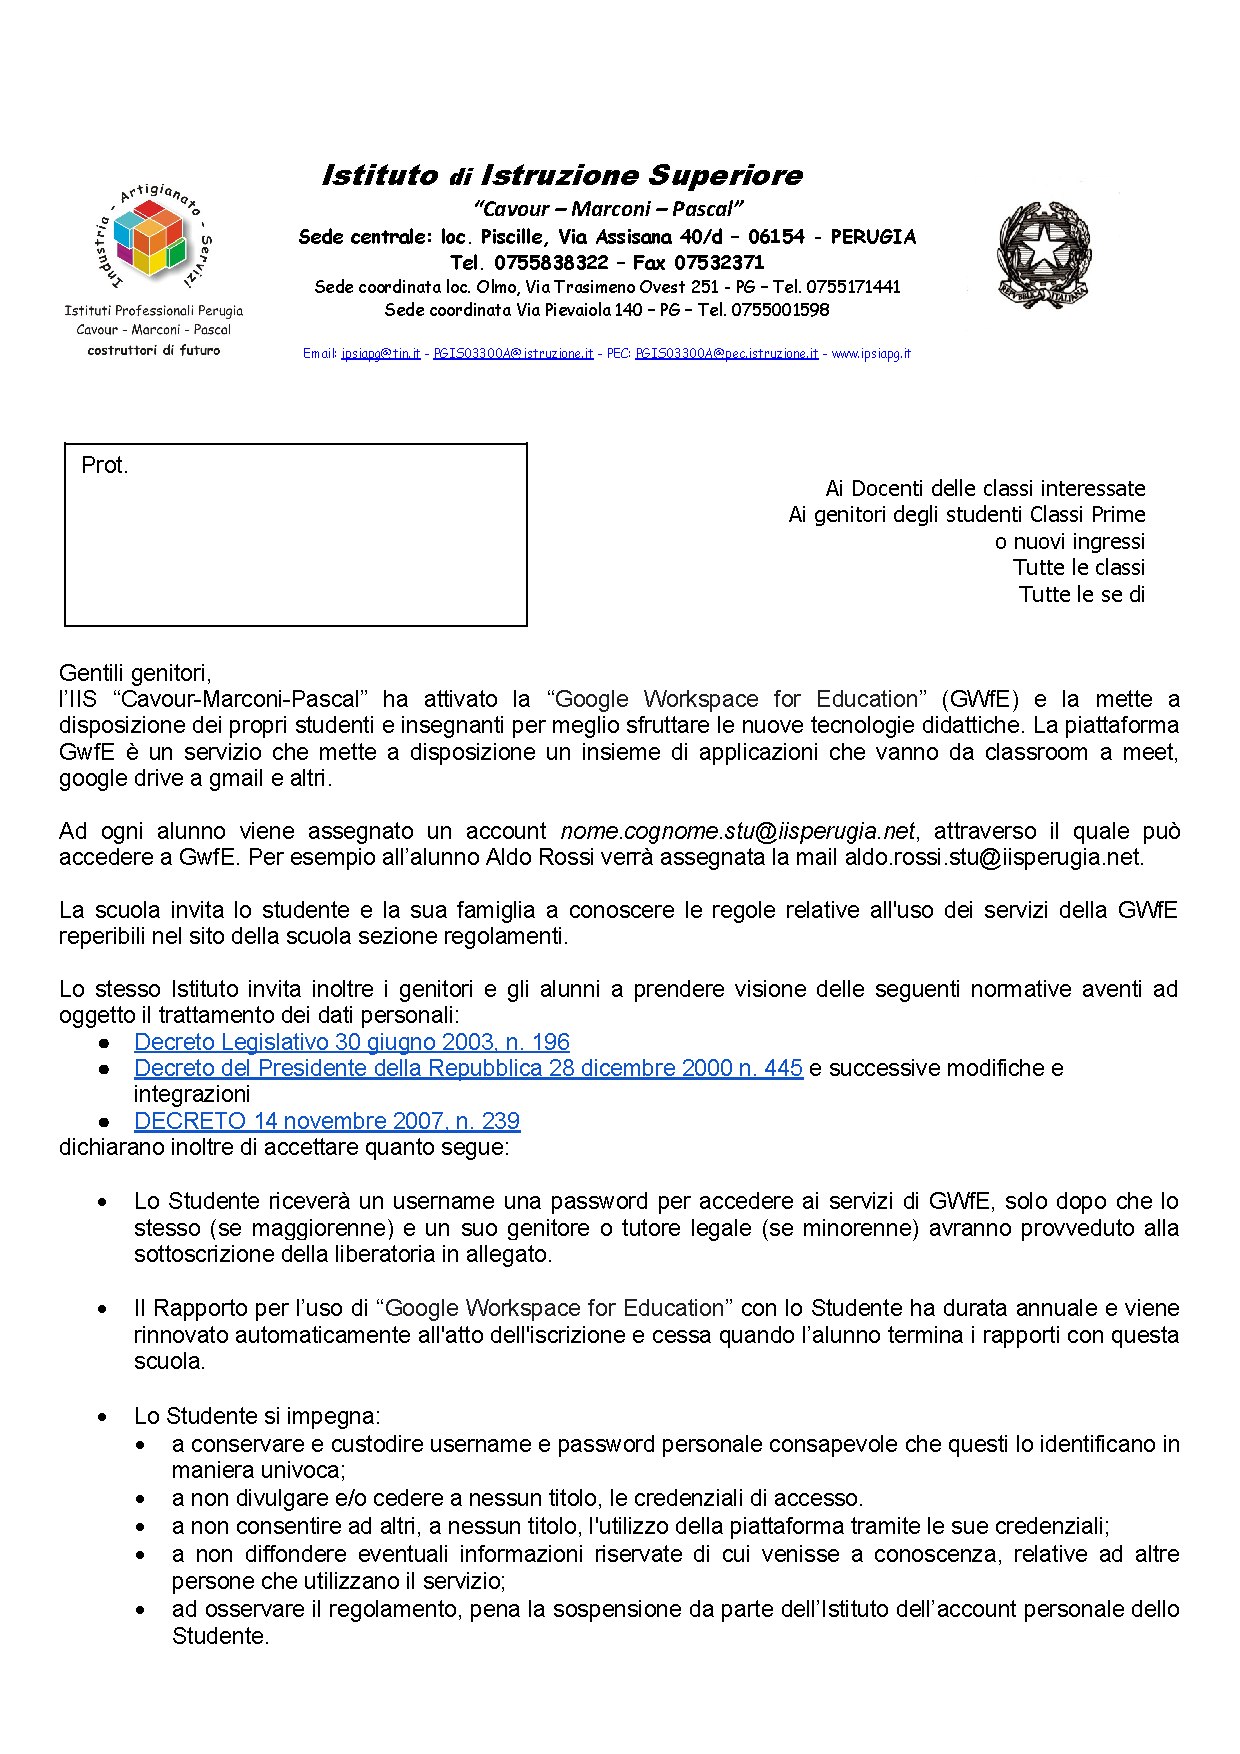
\includepdf[pages=1-2,addtotoc={1,section,1,Liberatoria Gsuite Scuola,pdf:autgsuit}]{NuovaAutorizzazioneGsuite.pdf}
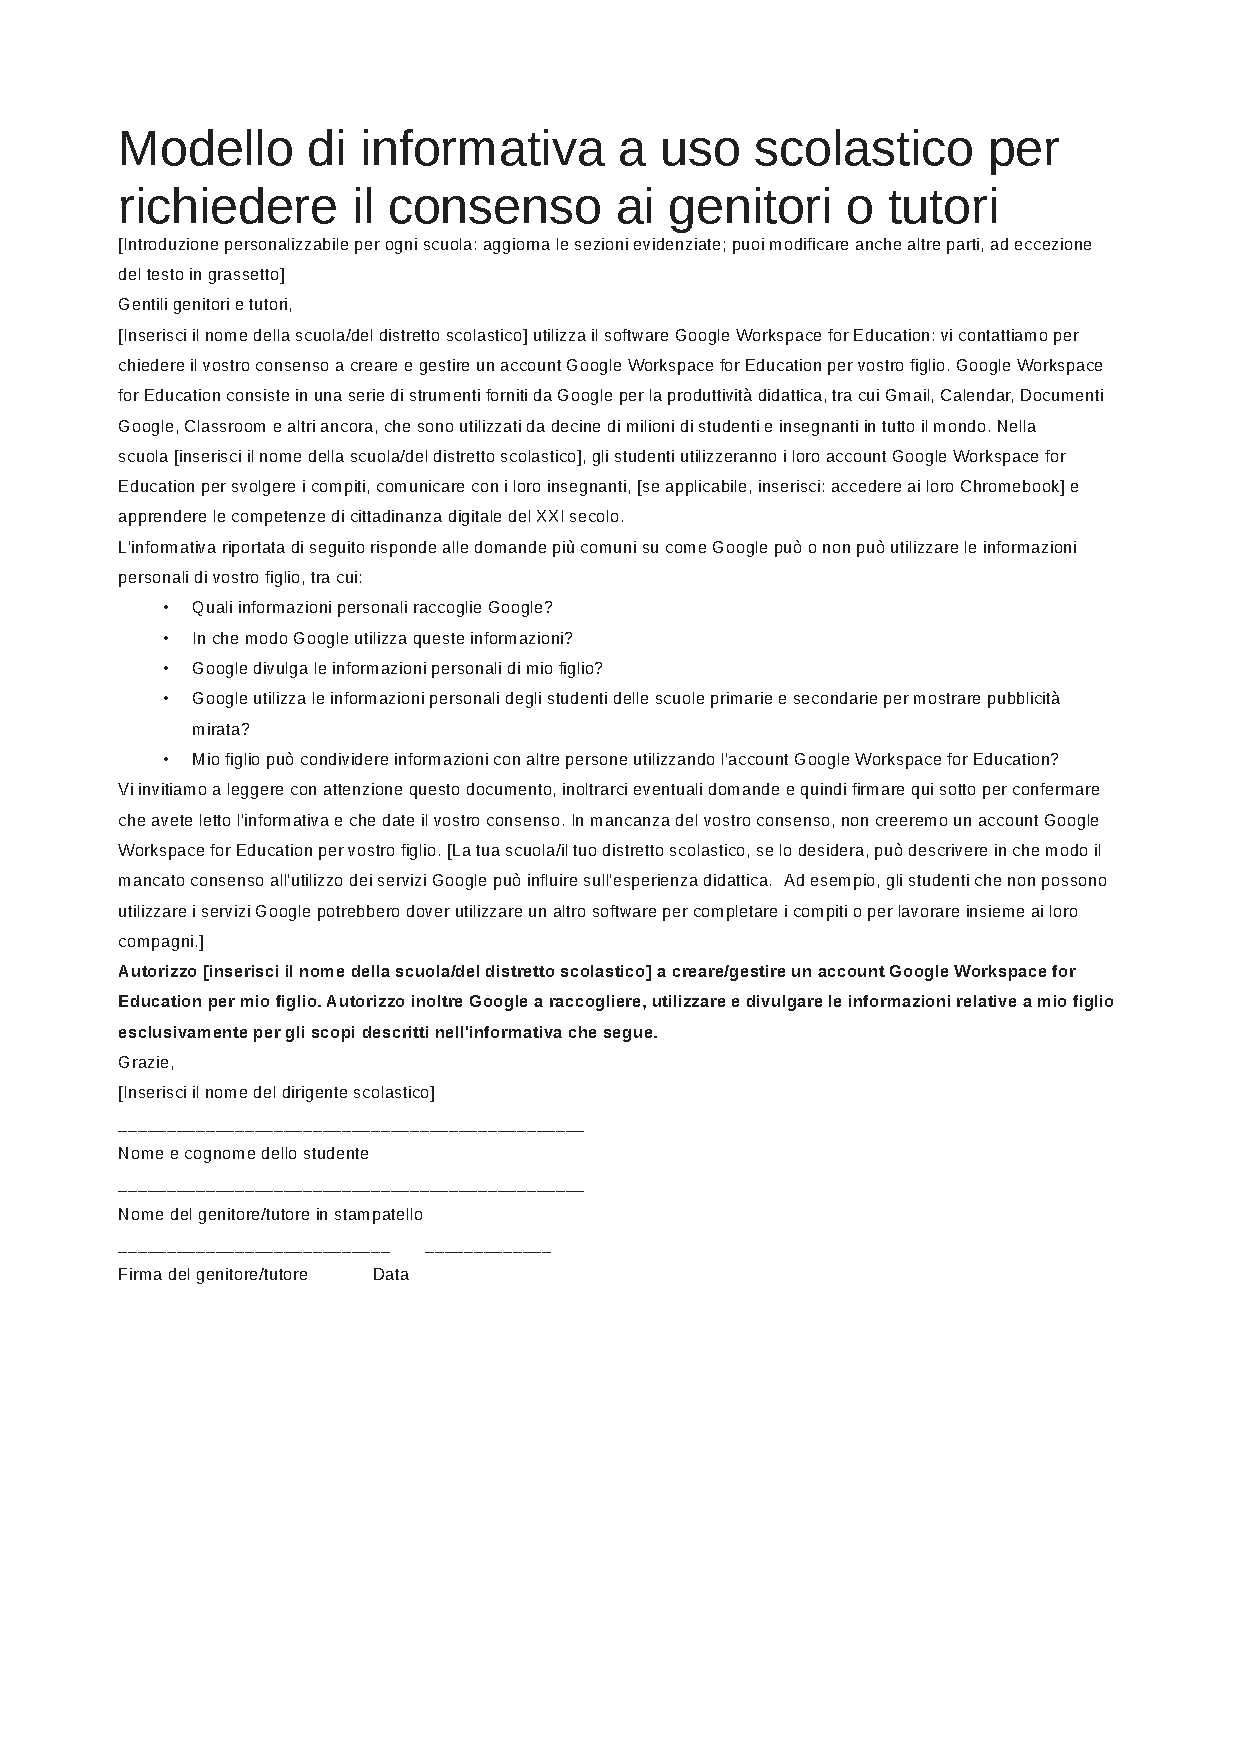
\includepdf[pages=1-4,addtotoc={1,section,1,Liberatoria Gsuite Scuola Google,pdf:autgsuitgoogle}]{liberatoriagoogle.pdf}
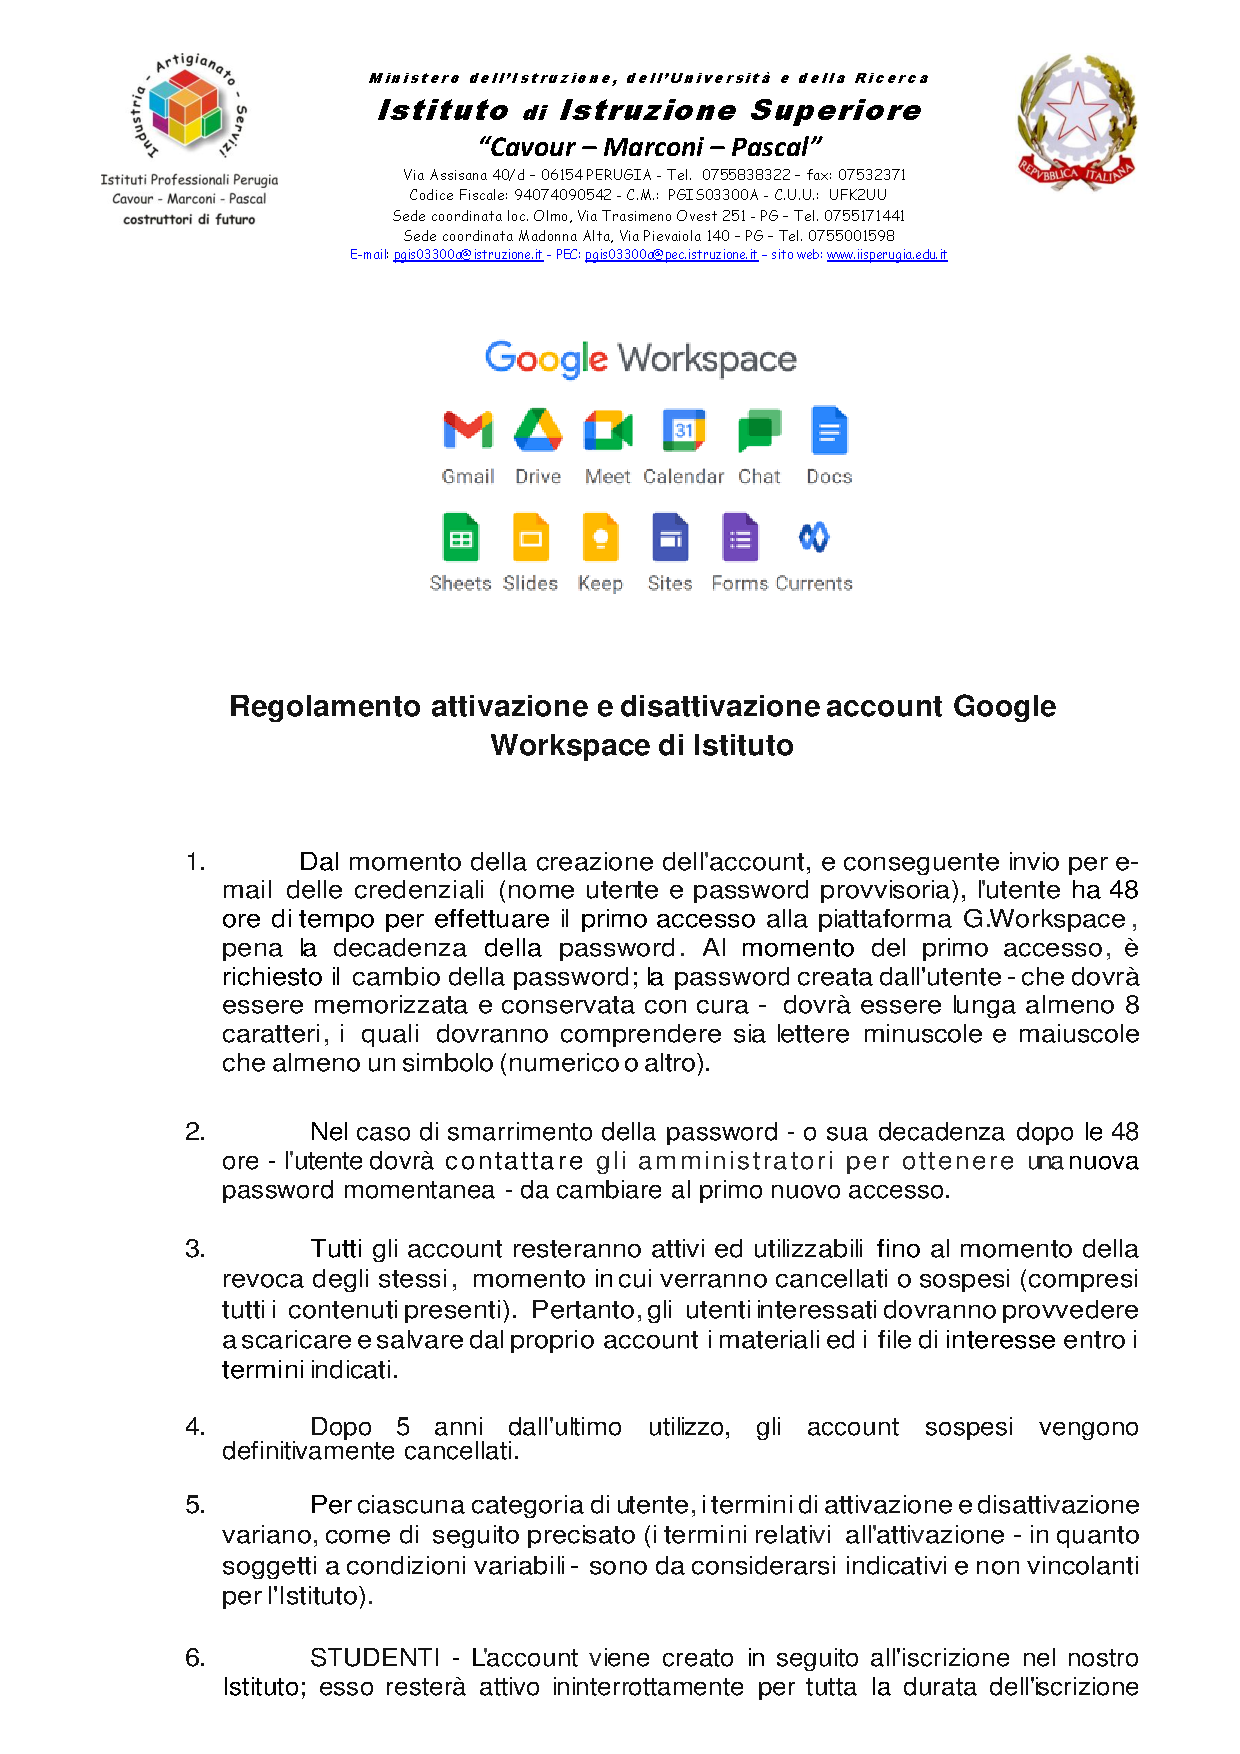
\includepdf[pages=1-3,addtotoc={1,section,1,Regolamento Google Workspace,pdf:autworkspace}]{RegolamentoGoogleWorkspaceIstituto.pdf}
\nocite{*}
\printbibliography[
heading=bibintoc,
title={Bibliografia}
]
\printindex
\end{document}